\documentclass{article}
\usepackage[utf8]{inputenc}
\usepackage{graphicx}

\title{Keterampilan Pemrograman}
\author{itsmeakil707 }
\date{October 2019}

\begin{document}
\title{Keterampilan Pemrograman}
\author{Akil Munawwar \\ 1184041 \\ D4 TI 1B }
\maketitle

\section{Output NPM}
\begin{enumerate}
    \item Jawaban No 1
    \begin{figure}[!htbp]
        \centering
        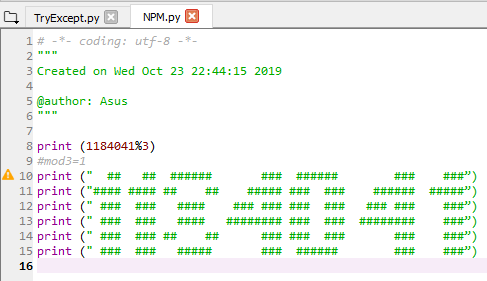
\includegraphics[scale=0.8]{NPM.PNG}
        \caption{NPM}
    \end{figure}
    \item Jawaban No 2
    \begin{figure}[!htbp]
        \centering
        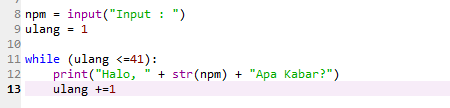
\includegraphics[scale=0.8]{PerulanganNPM.PNG}
        \caption{Perulangan NPM}
    \end{figure}
    \newpage
    \item Jawaban No 3
    \begin{figure}[!htbp]
        \centering
        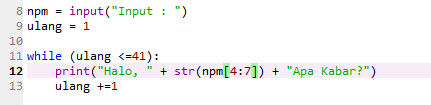
\includegraphics{PerulanganNPM2.PNG}
        \caption{Perulangan NPM 3 Angka Terakhir}
    \end{figure}
    \item Jawaban No 4
    \begin{figure}[!htbp]
        \centering
        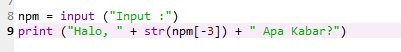
\includegraphics{PerulanganNPM3.PNG}
        \caption{Perulangan NPM Digit 3 Terakhir}
    \end{figure}
    \item Jawaban No 5
    \begin{figure}[!htbp]
        \centering
        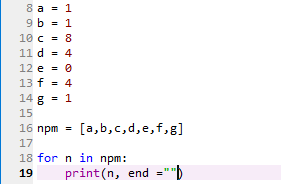
\includegraphics{PerulanganNPM4.PNG}
        \caption{Perulangan NPM Abjad}
    \end{figure}
    \newpage
    \item Jawaban No 6
    \begin{figure}[!htbp]
        \centering
        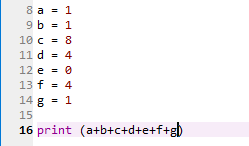
\includegraphics{PertambahanNPM.PNG}
        \caption{Pertambahan NPM}
    \end{figure}
    \item Jawaban No 7
    \begin{figure}[!htbp]
        \centering
        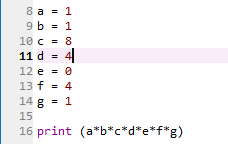
\includegraphics{PerkalianNPM.PNG}
        \caption{Perkalian NPM}
    \end{figure}
    \newpage
    \item Jawaban No 8
    \begin{figure}[!htbp]
        \centering
        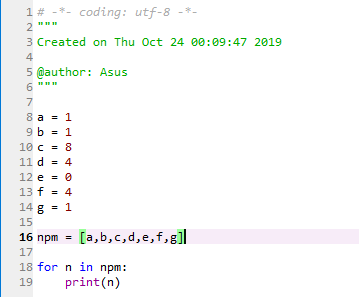
\includegraphics{Vertikal.PNG}
        \caption{Vertikal NPM}
    \end{figure}
    \item Jawaban No 9
    \begin{figure}[!htbp]
        \centering
        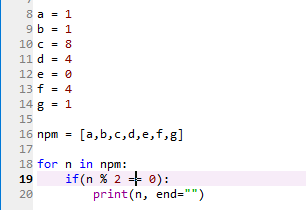
\includegraphics{GenapNPM.PNG}
        \caption{NPM Genap}
    \end{figure}
    \newpage
    \item Jawaban No 10
    \begin{figure}[!htbp]
        \centering
        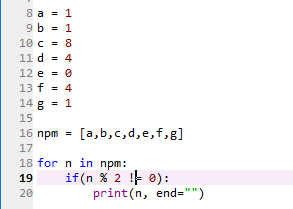
\includegraphics{GanjilNPM.PNG}
        \caption{NPM Ganjil}
    \end{figure}
    \item Jawaban No 11
    \begin{figure}[!htbp]
        \centering
        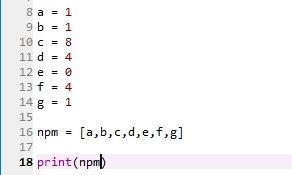
\includegraphics{PrimaNPM.PNG}
        \caption{Bilangan Prima NPM}
    \end{figure}
    \paragraph{} Disini, NPM saya tidak memiliki bilangan prima, maka dari itu saya hanya ngeprint NPM saja.
\end{enumerate}

\end{document}
